
\chapter*{The Continuity Equation}
\addcontentsline{toc}{chapter}{The Continuity Equation}
So far we have studied the numerical solution of partial differential equations one at a time, but in many interesting situations the problem to be solved involves coupled systems of differential equations. A "simple" example of such a system are the three coupled one-dimensional equations of gas dynamics. These are the equations of acoustics in a long tube with mass density $\rho(x, t)$, pressure $p(x, t)$, and gas velocity $v(x, t)$ as the dynamic variables. In the next lab we will tackle the hard problem of simultaneously advancing $\rho, T$, and $v$ in time and space, which will require three equations. But for now we will just practice on the continuity equation to develop the tools we need to do the full problem.
\section*{The Continuity Equation}
\addcontentsline{toc}{section}{The Continuity Equation}
The equation that enforces conservation of mass in acoustics is called the continuity equation:
\begin{equation}\label{eq:101}
\epsilon=\left|\frac{\text { Lhs }-\mathrm{Rhs}}{V_{\text {scale }}}\right|
\end{equation}
This equation says that as the gas particles are moved by the flow velocity $v(x, t)$, the density $\rho(x, t)$ is carried along with the flow and can be compressed or rarefied, but mass is not created or destroyed in this process.

Boundary conditions for the continuity equation are a bit different than we\rq ve encountered to this point. This is a convection equation, meaning that if you stand at a point in the flow, the solution at your location arrives (is convected to you) from further \rq\rq upwind.\lq\lq This has a strong effect on the boundary conditions. Suppose, for instance, that the flow field $v(x)$ is always positive, meaning that the wind is blowing to the right. At the left-hand boundary it makes sense to specify $\rho$ because somehow you might arrange to feed density in at that point so that it can be convected across the grid. But at the right boundary it makes no sense at all to specify a boundary condition because when the solution arrives there we just want to let the wind blow it away. (An exception to this rule occurs if $v=0$ at the boundary. In this case there is no wind to blow the solution from anywhere and it would be appropriate to specify a boundary condition.) We\rq ll try several approaches to represent these boundary conditions.

\begin{problem}\label{P10.1}
Let\rq s start with something really simple and inaccurate just to see what can
go wrong. If we use a nicely centered difference in $x$ and an inaccurate
forward difference in $t$, we find
\begin{equation}\label{eq:102}
\frac{\rho_{j}^{n+1}-\rho_{j}^{n}}{\tau}+\frac{1}{2 h}\left(\rho_{j+1}^{n} v_{j+1}-\rho_{j-1}^{n} v_{j-1}\right)=0
\end{equation}
Solve this equation for $\rho_{j}^{n+1}$ and use it in a time-advancing script like the one you built to do the wave equation in Lab 5. Use a cell-center grid with ghost points (use about 400 grid points). For initial conditions use
\begin{equation}\label{eq:103}
\rho(x, 0)=1+e^{-200(x / L-1 / 2)^{2}}
\end{equation}
with $ x \in[0, L], L=10$ , and


\begin{equation}\label{eq:104}
v(x)=v_0
\end{equation}
with $v_{0}=1$. At the left end use $\rho(0, t)=1$ and at the right end try the following two things:
\begin{enumerate}[label=(\roman*)]
\item Set a boundary condition: $\rho(L, t)=1$.
\item Just let mass leave by using linear extrapolation:
	\begin{equation}\label{eq:105}
\rho(L, t)=2 \rho(L-h, t)-\rho(L-2 h, t) \quad \text { or } \quad \rho_{N+1}=2 \rho_{N}-\rho_{N-1}
\end{equation}


\end{enumerate}
Run this algorithm with these two boundary conditions enough times, and with small enough time steps, that you become convinced that $\rho(L, t)=1$ is wrong and that the entire algorithm is worthless because it is unstable.\\
\end{problem}
As you might guess from the previous problem, the diffusion equation's simple appearance can be deceiving; it is one of the most difficult equations to solve numerically in all of computational physics because stable methods tend to be inaccurate and accurate methods tend either to be unstable, or non-conservative (as time runs mass spontaneously disappears), or unphysical (mass density and/or pressure become negative.)\\
Let\rq s try another method, known as the Lax-Wendroff method. The idea of the Lax-Wendroff algorithm is to use a Taylor series in time to obtain a second-order accurate method. Taylor expanding the density function in time gives us
\begin{equation}\label{eq:106}
\rho(x, t+\tau)=\rho(x, t)+\tau \frac{\partial \rho}{\partial t}+\frac{\tau^{2}}{2} \frac{\partial^{2} \rho}{\partial t^{2}}
\end{equation}
We can write the continuity equation as
\begin{equation}\label{eq:107}
\frac{\partial \rho}{\partial t}=-\frac{\partial}{\partial x}(\rho v)
\end{equation}
Substituting into our Taylor expansion then gives
\begin{equation}\label{eq:108}
\rho(x, t+\tau)=\rho(x, t)-\tau \frac{\partial}{\partial x}(\rho v)+\frac{\tau^{2}}{2} \frac{\partial}{\partial t}\left(-\frac{\partial}{\partial x}(\rho v)\right)
\end{equation}
If we reverse the order of the derivatives in the last term and assume that $v$ is not
a function of time, we can use Eq. \ref{eq:107} again to obtain.
\begin{equation}\label{eq:109}
\rho(x, t+\tau)=\rho(x, t)-\tau \frac{\partial \rho v}{\partial x}+\frac{\tau^{2}}{2} \frac{\partial}{\partial x}\left(v \frac{\partial \rho v}{\partial x}\right)
\end{equation}
Finally, we subtract $ρ(x,t)$ from both sides and divide by $\tau$ to obtain
\begin{equation}\label{eq:1010}
\frac{\rho(x, t+\tau)-\rho(x, t)}{\tau}=-\frac{\partial \rho v}{\partial x}+\frac{\tau}{2} \frac{\partial}{\partial x}\left(v \frac{\partial \rho v}{\partial x}\right)
\end{equation}
If we interpret the left-hand side as a time derivative, the second term on the right looks essentially like the diffusion equation. Since the equation we are solving is pure convection, the appearance of diffusion is not good news, but at least this algorithm is better than the horrible one in 10.1. Notice also that the diffusion coefficient in Eq. \ref{eq:101} is proportional to $\tau$ (stare at it until you can see that this is true), so if small time steps are being used diffusion won't hurt us too much.

\marginpar{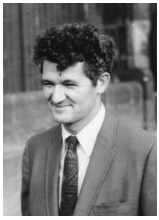
\includegraphics[width=\marginparwidth]{lax} \\ Peter Lax (b. 1926, American) Lax was the PhD advisor for Burton Wendroff.}
\begin{problem}\label{P10.2}
 Finite difference the expression in Eq. \ref{eq:1010} assuming that $v(x) = v0 =
const$, to find the Lax-Wendroff algorithm:
\begin{equation}\label{eq:1011}
\rho_{j}^{n+1}=\rho_{j}^{n}-\frac{v_{0} \tau}{2 h}\left(\rho_{j+1}^{n}-\rho_{j-1}^{n}\right)+\frac{v_{0}^{2} \tau^{2}}{2 h^{2}}\left(\rho_{j+1}^{n}-2 \rho_{j}^{n}+\rho_{j-1}^{n}\right)
\end{equation}
Change your script from $10.1$ to use the Lax-Wendroff algorithm. Again, use a cell-center grid with ghost points and about 400 grid points. Also use the same initial condition as in Problem $10.1$ and use the extrapolated boundary condition that just lets the pulse leave.\\
Show that Lax-Wendroff works pretty well unless the time step exceeds a Courant condition. Also show that it has the problem that the peak density slowly decreases as the density bump moves across the grid. (To see this use a relatively coarse grid and a time step just below the stability constraint.\\
Warning: do not run with $\tau=h / v_{0}$. If you do you will conclude that this algorithm is perfect, which is only true for this one choice of time step.) This problem is caused by the diffusive term in the algorithm, but since this diffusive term is the reason that this algorithm is not unstable like the one in 10.1, we suppose we should be grateful.
\end{problem}
\section*{Crank-Nicolson Again}
\addcontentsline{toc}{section}{Crank-Nicolson Again}

Finally, let\rq s try an implicit method, Crank-Nicolson in fact. As a reminder, the
continuity equation is
\begin{equation}\label{eq:1012}
\frac{\partial \rho}{\partial t}+\frac{\partial}{\partial x}(\rho v)=0
\end{equation}
We can\rq t solve this equation directly because it has two unknowns ( $\rho$ and $v$ ). But if we assume that $v$ is known, then it is possible to solve the equation using CrankNicolson. As usual for Crank-Nicolson, we forward difference in time and center difference in space to find
\begin{equation}\label{eq:1013}
\frac{\rho_{j}^{n+1}-\rho_{j}^{n}}{\tau}=-\frac{v_{j+1}^{n} \rho_{j+1}^{n}-v_{j-1}^{n} \rho_{j-1}^{n}}{2 h}
\end{equation}
Then we use time averaging to put the right side of the equation at the same time
level as the left (i.e. at the $n + 1/2$ time level):
\begin{equation}\label{eq:1014}
\rho_{j}^{n+1}-\rho_{j}^{n}=C_{1}\left(\rho_{j+1}^{n}+\rho_{j+1}^{n+1}\right)-C_{2}\left(\rho_{j-1}^{n}+\rho_{j-1}^{n+1}\right)
\end{equation}
where 
\begin{equation}\label{eq:1015}
C_{1}=-\frac{\tau}{8 h}\left(v_{j+1}^{n}+v_{j+1}^{n+1}\right)
\end{equation}
\begin{equation}\label{eq:1016}
C_{2}=-\frac{\tau}{8 h}\left(v_{j-1}^{n}+v_{j-1}^{n+1}\right)
\end{equation}
Then we put the $\rho^{n+1}$ terms on the left and the $\rho^n$ terms on the right:
\begin{equation}\label{eq:1017}
C_{2} \rho_{j-1}^{n+1}+\rho_{j}^{n+1}-C_{1} \rho_{j+1}^{n+1}=-C_{2} \rho_{j-1}^{n}+\rho_{j}^{n}+C_{1} \rho_{j+1}^{n}
\end{equation}
Then we write these equations along with the boundary conditions in matrix form
\begin{equation}\label{eq:1018}
\mathbf{A} \rho^{n+1}=\mathbf{B} \rho^{n}
\end{equation}
which we solve using linear algebra techniques. For this algorithm to calculate $\rho^{n+1}$, we need to feed it values for $\rho^{n}, v^{n}$, and $v^{n+1}$. For now, let\rq s side-step this issue by assuming that $v(x, t)$ is known, and a constant in time. In the next lab we\rq ll worry about advancing the velocity solution in parallel with the density.

\begin{problem}\label{P10.3}

	\marginpar{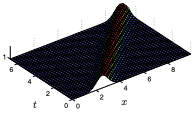
\includegraphics[width=\marginparwidth]{fig1001}\captionof{figure}{A pulse is convected across a region in which the convection velocity $v(x)$ is constant (Problem \ref{P10.3}(b)).}\label{fig:46}}
	\marginpar{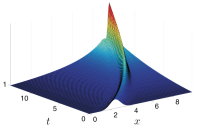
\includegraphics[width=\marginparwidth]{fig1002}\captionof{figure}{A pulse is convected across a region in which the convection velocity $v(x)$ is decreasing. Note that the pulse narrows and grows, conserving mass. (Prob$\operatorname{lem} 10.3(\mathrm{c}))$}\label{fig:47}}
\begin{enumerate}[label=(\alph*)]
\item  Write a program that implements this algorithm, perhaps starting from one of your programs from the Schr{\"o}dinger equation lab. Work out how to implement the boundary conditions, $\rho(0, t)=1$ and $\rho(L, t)$ is just allowed to leave, by properly defining the top and bottom rows of the matrices $\mathbf{A}$ and $\mathbf{B}$. This involves multiplying $\mathbf{B} \rho^{n}$ to find an $r$-vector as you have done before.
\item  Implement this algorithm with a constant convection velocity $v=$ $v_{0}$ and show that the algorithm conserves amplitude to very high precision and does not widen due to diffusion. These two properties make this algorithm a good one as long as shock waves don\rq t develop.
\item Now use a convection velocity that varies with $x$ :
\begin{equation}\label{eq:1019}
v(x)=1.2-x / L
\end{equation}
This velocity slows down as the flow moves to the right, which means
that the gas in the back is moving faster than the gas in the front,
causing compression and an increase in density. You should see the
slowing down of the pulse and the increase in density in your numerical solution.
\item Go back to a constant convection velocity $v = v_0$ and explore the way
this algorithm behaves when we have a shock wave (discontinuous
density) by using as the initial condition
\begin{equation}\label{eq:1020}
\rho(x, 0)= \begin{cases}1.0 & \text { if } 0 \leq x \leq L / 2 \\ 0 & \text { otherwise }\end{cases}
\end{equation}
The true solution of this problem just convects the step to the right;
you will find that Crank-Nicolson fails at this seemingly simple task.
\item For comparison, try the same step-function initial condition in your
Lax-Wendroff script from Problem \ref{P10.2}.
\end{enumerate}
\end{problem}
Our Crank-Nicolson algorithm is both stable and conservative, but it only
works well if the solution doesn\rq t become too steep. This is a severe limitation,
since we are talking about gas dynamics here and shock waves routinely show up
as solutions in gas dynamics. Numerical methods that properly handle shocks
are much more involved than the ones we will show you here.
